% !TeX program = xelatex
\documentclass[a4paper,10pt]{article}

% ============================================================================
% កញ្ចប់បណ្ណាល័យ (Packages) – តាមលំនាំស្តង់ដារអនុវិទ្យាល័យព្រះក្រសាំង (ls_plan.tex)
% ============================================================================
\usepackage[a4paper, left=0.95cm, right=0.95cm, top=0.85cm, bottom=0.92cm, footskip=0.52cm]{geometry}
\usepackage{amsmath}
\usepackage{unicode-math}
\usepackage{fontspec}
\usepackage{array, longtable, multirow, colortbl}
\usepackage[table]{xcolor}
\usepackage{enumitem}
\usepackage{pifont}
\usepackage{fancyhdr}
\usepackage{tikz}
\usetikzlibrary{calc, arrows.meta, angles, quotes, decorations.markings, babel}

% LaTeX 2025 + longtable compatibility guard
\makeatletter
\let\@expl@@@mark@update@singlecol@structures@@\relax
\makeatother

% ============================================================================
% ការកំណត់ពុម្ពអក្សរ (Cross-Platform Windows + Linux Cloud fonts/)
% ============================================================================
\providecommand{\NGSFindFonts}{%
  \IfFileExists{C:/Windows/Fonts/cambria.ttc}{%
    \def\NGSSysPath{C:/Windows/Fonts/}%
    \def\NGSUserPath{C:/Users/KIT/AppData/Local/Microsoft/Windows/Fonts/}%
  }{%
    \IfFileExists{./fonts/KhmerOSsiemreap.ttf}{\def\NGSSysPath{./fonts/}\def\NGSUserPath{./fonts/}}{%
    \IfFileExists{../fonts/KhmerOSsiemreap.ttf}{\def\NGSSysPath{../fonts/}\def\NGSUserPath{../fonts/}}{%
    \IfFileExists{../../fonts/KhmerOSsiemreap.ttf}{\def\NGSSysPath{../../fonts/}\def\NGSUserPath{../../fonts/}}{%
    \IfFileExists{../../../fonts/KhmerOSsiemreap.ttf}{\def\NGSSysPath{../../../fonts/}\def\NGSUserPath{../../../fonts/}}{%
    \IfFileExists{../../../../fonts/KhmerOSsiemreap.ttf}{\def\NGSSysPath{../../../../fonts/}\def\NGSUserPath{../../../../fonts/}}{%
    \IfFileExists{../../../../../fonts/KhmerOSsiemreap.ttf}{\def\NGSSysPath{../../../../../fonts/}\def\NGSUserPath{../../../../../fonts/}}{%
    \IfFileExists{../../../../../../fonts/KhmerOSsiemreap.ttf}{\def\NGSSysPath{../../../../../../fonts/}\def\NGSUserPath{../../../../../../fonts/}}{%
      \def\NGSSysPath{../../../../../../../fonts/}\def\NGSUserPath{../../../../../../../fonts/}%
    }}}}}}}%
  }%
}
\NGSFindFonts

\setmathfont[
  Path={\NGSSysPath},
  FontIndex=1,
  Scale=1.02
]{cambria.ttc}

\defaultfontfeatures{Ligatures=TeX}

\setmainfont[
  Path={\NGSUserPath},
  Extension=.ttf,
  Script=Khmer,
  BoldFont={KhmerOSsiemreap},
  BoldFeatures={FakeBold=1.8},
  ItalicFont={KhmerOSsiemreap},
  ItalicFeatures={FakeSlant=0.25},
  BoldItalicFont={KhmerOSsiemreap},
  BoldItalicFeatures={FakeBold=1.8, FakeSlant=0.25}
]{KhmerOSsiemreap}

\newfontfamily\muol[
  Path={\NGSUserPath},
  Extension=.ttf,
  Script=Khmer
]{KhmerOSmuollight}

\newfontfamily\TimesEn[
  Path={\NGSSysPath},
  Extension=.ttf,
  Scale=1.00,
  BoldFont={timesbd},
  ItalicFont={timesi},
  BoldItalicFont={timesbi}
]{times}

\newfontfamily\NagaBold[
  Path={\NGSUserPath},
  Extension=.ttf
]{AKbalthom Naga Bold}

\newfontfamily\CalibriFont[
  Path={\NGSSysPath},
  Extension=.ttf
]{calibri}

\newfontfamily\Tacteing[
  Path={\NGSUserPath}
]{TACTENG.TTF}

\newfontfamily\CourierBullet[
  Path={\NGSSysPath},
  Extension=.ttf
]{cour}
\newcommand{\wcirc}{{\CourierBullet\fontsize{9.5pt}{11pt}\selectfont o}}

\XeTeXlinebreaklocale "km"
\XeTeXlinebreakskip = 0pt plus 1pt minus 0.1pt

% ============================================================================
% ពណ៌ និងទម្រង់ទំព័រ
% ============================================================================
\definecolor{stepgray}{HTML}{D9D9D9}
\definecolor{headgray}{HTML}{F2F2F2}
\definecolor{boxgray}{HTML}{E6E6E6}
\definecolor{darkred}{HTML}{C00000}
\definecolor{red5e}{HTML}{FF0000}

\pagestyle{fancy}
\fancyhf{}
\renewcommand{\headrulewidth}{0pt}
\fancyfoot[R]{\CalibriFont\fontsize{11pt}{13pt}\selectfont\thepage}

\setlength{\parindent}{0pt}
\setlength{\parskip}{0pt}
\setlength{\tabcolsep}{3.8pt}

\newcolumntype{L}[1]{>{\raggedright\arraybackslash}p{#1}}

% ============================================================================
% ម៉ាក្រូជំនួយ (Helper Macros)
% ============================================================================
\newcommand{\en}[1]{{\TimesEn #1}}
\newcommand{\enbf}[1]{{\TimesEn\textbf{#1}}}
\newcommand{\unit}[1]{\,\text{\en{#1}}}
\newcommand{\fiveE}[1]{{\NagaBold\fontsize{9.5pt}{13pt}\selectfont\textcolor{red5e}{#1}}}
\newcommand{\timenote}[1]{\textcolor{darkred}{\textit{#1}}}
\newcommand{\graybox}[1]{\colorbox{boxgray}{\strut\hspace{2pt}#1\hspace{2pt}}}
\newcommand{\ditem}{\tikz[baseline=-0.5ex]\fill (0,0.42ex) -- (0.42ex,0) -- (0,-0.42ex) -- (-0.42ex,0) -- cycle;\hspace{0.3em}}
\newcommand{\cnum}[1]{{\fontsize{10.5pt}{12pt}\selectfont\ding{\numexpr181+#1\relax}}\hspace{0.2em}}
\newcommand{\cfig}[1]{\par\vspace{4pt}{\centering #1\par}\vspace{4pt}}
\newcommand{\stepheader}[1]{\multicolumn{3}{|c|}{\cellcolor{stepgray}\muol #1} \\* \noalign{\hrule height 0.4pt}}
\newcommand{\tri}[1]{\ensuremath{\triangle #1}}
\newcommand{\ang}[1]{\ensuremath{\angle #1}}
\newcommand{\cg}{\ensuremath{\cong}}
\newcommand{\chkbox}{\tikz[baseline=-0.15ex]\draw[black, line width=0.8pt] (0,0) rectangle (0.23cm,0.23cm);}

\tikzset{
  tk1/.style={postaction={decorate},decoration={markings,mark=at position 0.50 with {\draw[black, line width=0.85pt](0,-0.095)--(0,0.095);}}},
  tk2/.style={postaction={decorate},decoration={markings,
    mark=at position 0.45 with {\draw[black, line width=0.85pt](0,-0.095)--(0,0.095);},
    mark=at position 0.55 with {\draw[black, line width=0.85pt](0,-0.095)--(0,0.095);}}},
  tk3/.style={postaction={decorate},decoration={markings,
    mark=at position 0.42 with {\draw[black, line width=0.85pt](0,-0.095)--(0,0.095);},
    mark=at position 0.50 with {\draw[black, line width=0.85pt](0,-0.095)--(0,0.095);},
    mark=at position 0.58 with {\draw[black, line width=0.85pt](0,-0.095)--(0,0.095);}}}
}

\newcommand{\rightbox}[4][0.19]{%
  \draw[black, line width=0.8pt]
    ($(#3)!#1!(#2)$) -- ($($(#3)!#1!(#2)$)+($(#3)!#1!(#4)$)-(#3)$) -- ($(#3)!#1!(#4)$);
}

\newcommand{\khmflourish}{{\Tacteing\fontsize{36pt}{14pt}\selectfont\raisebox{-5pt}{3}}}

% ============================================================================
% ម៉ាក្រូគូសរូបធរណីមាត្រ B&W ច្បាស់សមាមាត្រ (3.8–6.8 cm, អក្សរខ្មៅ 100%)
% ============================================================================

% ១. រំលឹកមេរៀនចាស់៖ (ក) មេដ្យាន vs កម្ពស់ និង (ខ) បាតមធ្យមត្រីកោណ
\newcommand{\figPrereqMED}{%
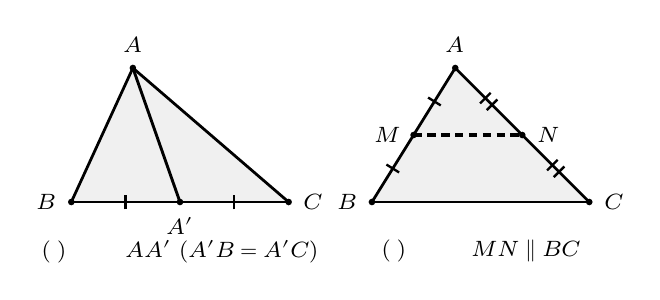
\begin{tikzpicture}[scale=0.92, every node/.style={font=\footnotesize, text=black}]
  % (១) មេដ្យាន AA'
  \begin{scope}[shift={(0,0)}]
    \coordinate (B) at (0,0);
    \coordinate (C) at (3.0,0);
    \coordinate (A) at (0.85,1.85);
    \coordinate (Ap) at (1.50,0);
    \fill[gray!12] (A) -- (B) -- (C) -- cycle;
    \draw[black, line width=1.0pt] (A) -- (B) (A) -- (C);
    \draw[black, line width=1.0pt, tk1] (B) -- (Ap);
    \draw[black, line width=1.0pt, tk1] (Ap) -- (C);
    \draw[black, line width=1.05pt] (A) -- (Ap);
    \fill[black] (A) circle (1.3pt) node[above=2pt] {$A$};
    \fill[black] (B) circle (1.3pt) node[left=2pt] {$B$};
    \fill[black] (C) circle (1.3pt) node[right=2pt] {$C$};
    \fill[black] (Ap) circle (1.3pt) node[below=2pt] {$A'$};
    \node at (1.50,-0.68) {(១) មេដ្យាន $AA'$ ($A'B=A'C$)};
  \end{scope}
  % (២) បាតមធ្យម MN || BC
  \begin{scope}[shift={(4.15,0)}]
    \coordinate (B) at (0,0);
    \coordinate (C) at (3.0,0);
    \coordinate (A) at (1.15,1.85);
    \coordinate (M) at ($(A)!0.5!(B)$);
    \coordinate (N) at ($(A)!0.5!(C)$);
    \fill[gray!12] (A) -- (B) -- (C) -- cycle;
    \draw[black, line width=1.0pt, tk1] (A) -- (M);
    \draw[black, line width=1.0pt, tk1] (M) -- (B);
    \draw[black, line width=1.0pt, tk2] (A) -- (N);
    \draw[black, line width=1.0pt, tk2] (N) -- (C);
    \draw[black, line width=1.0pt] (B) -- (C);
    \draw[black, line width=1.1pt, densely dashed] (M) -- (N);
    \fill[black] (A) circle (1.3pt) node[above=2pt] {$A$};
    \fill[black] (B) circle (1.3pt) node[left=2pt] {$B$};
    \fill[black] (C) circle (1.3pt) node[right=2pt] {$C$};
    \fill[black] (M) circle (1.3pt) node[left=2pt] {$M$};
    \fill[black] (N) circle (1.3pt) node[right=2pt] {$N$};
    \node at (1.50,-0.68) {(២) បាតមធ្យម $MN \parallel BC$};
  \end{scope}
\end{tikzpicture}}

% ២. E1 Engage: បន្ទះតុឈើរាងត្រីកោណដាក់ជើងទម្រតែមួយត្រង់ G
\newcommand{\figEngageMED}{%
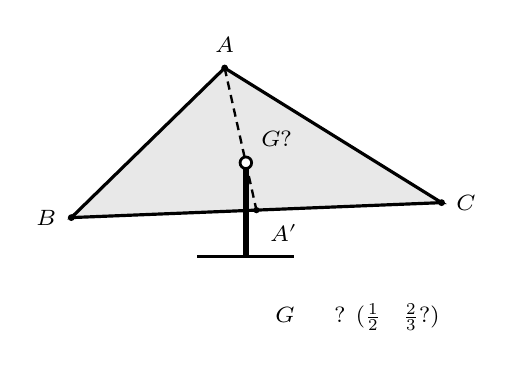
\begin{tikzpicture}[scale=0.95, every node/.style={font=\footnotesize, text=black}]
  \coordinate (B) at (-2.40,-0.35);
  \coordinate (C) at (2.55,-0.15);
  \coordinate (A) at (-0.35,1.65);
  \coordinate (Ap) at ($(B)!0.5!(C)$);
  \coordinate (G) at ($0.3333*(A)+0.3333*(B)+0.3333*(C)$);
  \fill[gray!18] (A) -- (B) -- (C) -- cycle;
  \draw[black, line width=1.15pt] (A) -- (B) -- (C) -- cycle;
  \draw[black, line width=0.85pt, densely dashed] (A) -- (Ap);
  % ជើងទម្រតុក្រោម G
  \draw[black, line width=2.2pt] (G) -- ($(G)+(0,-1.25)$);
  \draw[black, line width=1.2pt] ($(G)+(-0.65,-1.25)$) -- ($(G)+(0.65,-1.25)$);
  \fill[black] (A) circle (1.3pt) node[above=2pt] {$A$};
  \fill[black] (B) circle (1.3pt) node[left=2pt] {$B$};
  \fill[black] (C) circle (1.3pt) node[right=2pt] {$C$};
  \fill[black] (Ap) circle (1.2pt) node[below right=1.5pt] {$A'$};
  \fill[white] (G) circle (2.2pt);
  \draw[black, line width=1.0pt] (G) circle (2.2pt);
  \node[above right=2pt] at (G) {$G?$};
  \node at (0.05,-1.68) {បន្ទះតុត្រីកោណមានលំនឹងត្រង់ចំណុច $G$ មួយណា? ($\frac{1}{2}$ ឬ $\frac{2}{3}$?)};
\end{tikzpicture}}

% ៣. E2 សម្រាយបញ្ជាក់ឧទាហរណ៍សៀវភៅគោល (ទំ.២០៥)៖ ប្រលេឡូក្រាម BDCG
\newcommand{\figProofMED}{%
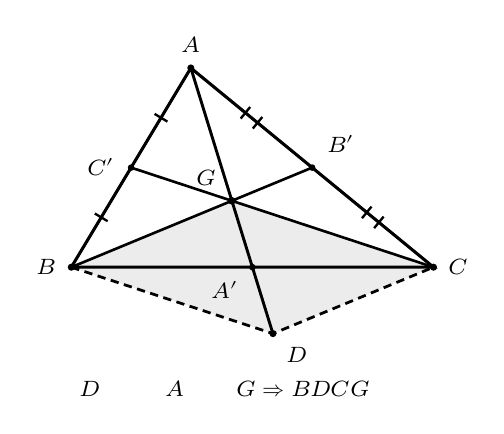
\begin{tikzpicture}[scale=0.92, every node/.style={font=\footnotesize, text=black}]
  \coordinate (A) at (-0.65,2.75);
  \coordinate (B) at (-2.30,0);
  \coordinate (C) at (2.70,0);
  \coordinate (Ap) at ($(B)!0.5!(C)$);
  \coordinate (Bp) at ($(A)!0.5!(C)$);
  \coordinate (Cp) at ($(A)!0.5!(B)$);
  \coordinate (G) at ($0.3333*(A)+0.3333*(B)+0.3333*(C)$);
  \coordinate (D) at ($2*(G)-(A)$);

  \fill[gray!15] (B) -- (D) -- (C) -- (G) -- cycle;
  \draw[black, line width=1.1pt] (A) -- (B) -- (C) -- cycle;
  \draw[black, line width=0.95pt] (B) -- (Bp) (C) -- (Cp);
  \draw[black, line width=1.05pt] (A) -- (D);
  \draw[black, line width=1.0pt, densely dashed] (B) -- (D) -- (C);

  % សញ្ញាឆ្នូតចំណុចកណ្ដាល
  \draw[black, line width=0.8pt, tk1] (A) -- (Cp);
  \draw[black, line width=0.8pt, tk1] (Cp) -- (B);
  \draw[black, line width=0.8pt, tk2] (A) -- (Bp);
  \draw[black, line width=0.8pt, tk2] (Bp) -- (C);

  \fill[black] (A) circle (1.4pt) node[above=2pt] {$A$};
  \fill[black] (B) circle (1.4pt) node[left=2pt] {$B$};
  \fill[black] (C) circle (1.4pt) node[right=2pt] {$C$};
  \fill[black] (Cp) circle (1.3pt) node[left=2.5pt] {$C'$};
  \fill[black] (Bp) circle (1.3pt) node[above right=2pt] {$B'$};
  \fill[black] (Ap) circle (1.3pt) node[below left=1.5pt] {$A'$};
  \fill[black] (G) circle (1.5pt) node[above left=2pt] {$G$};
  \fill[black] (D) circle (1.4pt) node[below right=1.5pt] {$D$};
  \node at (0.20,-1.68) {ចំណុច $D$ ឆ្លុះនឹង $A$ ធៀបនឹង $G \Rightarrow BDCG$ ជាប្រលេឡូក្រាម};
\end{tikzpicture}}

% ៤. E4 លំហាត់គំរូ (BB'=CC') និង ប្រតិបត្តិសង់កំពូល C (ទំ.២០៦)
\newcommand{\figElaborateMED}{%
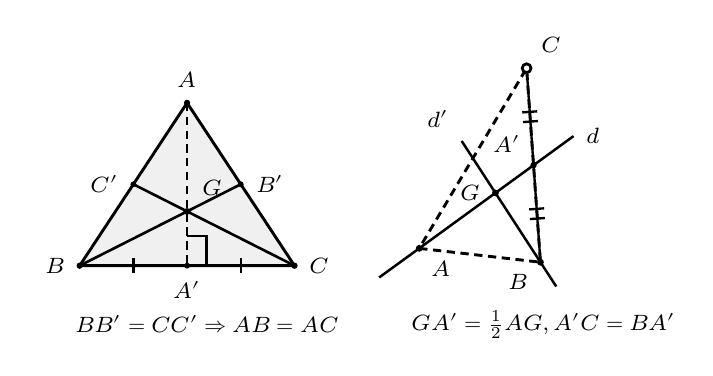
\begin{tikzpicture}[scale=0.88, every node/.style={font=\footnotesize, text=black}]
  % (ក) លំហាត់គំរូ BB' = CC'
  \begin{scope}[shift={(0,0)}]
    \coordinate (B) at (-1.55,0);
    \coordinate (C) at (1.55,0);
    \coordinate (A) at (0,2.35);
    \coordinate (Ap) at (0,0);
    \coordinate (Bp) at ($(A)!0.5!(C)$);
    \coordinate (Cp) at ($(A)!0.5!(B)$);
    \coordinate (G) at (0,0.783);
    \fill[gray!12] (A) -- (B) -- (C) -- cycle;
    \draw[black, line width=1.05pt] (A) -- (B) -- (C) -- cycle;
    \draw[black, line width=0.95pt] (B) -- (Bp) (C) -- (Cp);
    \draw[black, line width=1.0pt, densely dashed] (A) -- (Ap);
    \rightbox[0.18]{A}{Ap}{C}
    \draw[black, line width=0.8pt, tk1] (B) -- (Ap);
    \draw[black, line width=0.8pt, tk1] (Ap) -- (C);
    \fill[black] (A) circle (1.3pt) node[above=2pt] {$A$};
    \fill[black] (B) circle (1.3pt) node[left=2pt] {$B$};
    \fill[black] (C) circle (1.3pt) node[right=2pt] {$C$};
    \fill[black] (Cp) circle (1.2pt) node[left=2pt] {$C'$};
    \fill[black] (Bp) circle (1.2pt) node[right=2pt] {$B'$};
    \fill[black] (Ap) circle (1.2pt) node[below=2pt] {$A'$};
    \fill[black] (G) circle (1.4pt) node[above right=2pt] {$G$};
    \node at (0,-0.85) {គំរូ៖ $BB'=CC' \Rightarrow AB=AC$};
  \end{scope}
  % (ខ) ប្រតិបត្តិ សង់កំពូល C ស្គាល់ d, d' និង A, B
  \begin{scope}[shift={(4.45,0)}]
    \coordinate (G) at (0,1.05);
    \coordinate (A) at (-1.10,0.25);
    \coordinate (Ap) at ($(G)+0.5*(G)-0.5*(A)$);
    \coordinate (B) at (0.65,0.05);
    \coordinate (C) at ($2*(Ap)-(B)$);
    \draw[black, line width=0.9pt] ($(A)!-0.35!(Ap)$) -- ($(A)!1.35!(Ap)$) node[right=1pt] {$d$};
    \draw[black, line width=0.9pt] ($(B)!-0.35!(G)$) -- ($(B)!1.75!(G)$) node[above left=1pt] {$d'$};
    \draw[black, line width=1.05pt, densely dashed] (A) -- (B) -- (C) -- cycle;
    \draw[black, line width=0.85pt, tk2] (B) -- (Ap);
    \draw[black, line width=0.85pt, tk2] (Ap) -- (C);
    \fill[black] (A) circle (1.4pt) node[below right=1pt] {$A$};
    \fill[black] (B) circle (1.4pt) node[below left=1pt] {$B$};
    \fill[black] (G) circle (1.4pt) node[left=2pt] {$G$};
    \fill[black] (Ap) circle (1.3pt) node[above left=1pt] {$A'$};
    \fill[white] (C) circle (1.8pt);
    \draw[black, line width=1.0pt] (C) circle (1.8pt);
    \node[above right=2pt] at (C) {$C$};
    \node at (0.15,-0.85) {ប្រតិបត្តិ៖ $GA'=\frac{1}{2}AG, A'C=BA'$};
  \end{scope}
\end{tikzpicture}}

% ============================================================================
% ចាប់ផ្ដើមឯកសារ (Document Body)
% ============================================================================
\begin{document}
\fontsize{10pt}{15.2pt}\selectfont

% -------------------- ក្បាលកិច្ចតែងការ (Header) --------------------
\begin{center}
  {\muol\fontsize{11pt}{16pt}\selectfont ព្រះរាជាណាចក្រកម្ពុជា}\\[2pt]
  {\muol\fontsize{10pt}{15pt}\selectfont ជាតិ សាសនា ព្រះមហាក្សត្រ}\\[1pt]
  \khmflourish
\end{center}

\vspace{-26pt}
{\muol\fontsize{9.5pt}{12.8pt}\selectfont
មន្ទីរអប់រំ យុវជន និងកីឡា ខេត្តកំពង់ធំ\\
ការិយាល័យអប់រំ យុវជន និងកីឡា ស្រុកកំពង់ស្វាយ\\
អនុវិទ្យាល័យព្រះក្រសាំង}

\vspace{1pt}
\begin{center}
  {\muol\fontsize{10pt}{14.5pt}\selectfont កិច្ចតែងការបង្រៀន}
\end{center}
\vspace{0pt}

% -------------------- ព័ត៌មានទូទៅ (Metadata) --------------------
{\renewcommand{\arraystretch}{0.98}
\hspace*{4.05cm}%
\begin{tabular}{@{}l l l@{}}
  - \hspace{0.35cm} មុខវិជ្ជា & : & គណិតវិទ្យា ថ្នាក់ទី៨ \\
  - \hspace{0.35cm} ចំណងជើងមេរៀន & : & មេរៀនទី១៦ បន្ទាត់និងអង្កត់ពិសេសជួបគ្នានៅក្នុងត្រីកោណ \\
  - \hspace{0.35cm} ចំណងជើងរង & : & ១៦.១ លក្ខណៈមេដ្យាននៃត្រីកោណ (ទំព័រ ២០៥--២០៦) \\
  - \hspace{0.35cm} រយៈពេល & : & ១ ម៉ោងសិក្សា (៥០ នាទី) \\
  - \hspace{0.35cm} បង្រៀនដោយ & : & ហុក ប៊ុនថែន \\
  - \hspace{0.35cm} កាលបរិច្ឆេទ & : & ថ្ងៃ\makebox[18mm]{\dotfill}\ ទី\makebox[8mm]{\dotfill}\ ខែ\makebox[18mm]{\dotfill}\ ឆ្នាំ២០២៦ \\
\end{tabular}

\vspace{2pt}

% -------------------- I. វត្ថុបំណង --------------------
\textbf{I.} {\muol វត្ថុបំណង}\\[1pt]
\hspace*{0.55cm}%
\begin{tabular}{@{}l l L{14.2cm}@{}}
  \wcirc \hspace{0.25cm} វិជ្ជាសម្បទា & : & សិស្សប្រាប់បានត្រឹមត្រូវពីនិយមន័យទីប្រជុំទម្ងន់ $G$ និងទ្រឹស្តីបទលក្ខណៈមេដ្យានទាំងបីនៃត្រីកោណ ($AG=\frac{2}{3}AA', GA'=\frac{1}{3}AA', AG=2GA'$) តាមរយៈការវាស់ស្ទង់និងសម្រាយបញ្ជាក់លើសន្លឹកកិច្ចការ ។ \\
  \wcirc \hspace{0.25cm} បំណិនសម្បទា & : & សិស្សគណនាប្រវែងកំណាត់មេដ្យាន ស្រាយបញ្ជាក់លក្ខណៈត្រីកោណសមបាតពេលមេដ្យានពីរស្មើគ្នា ($BB'=CC'$) និងសង់កំពូលទីបី $C$ នៃត្រីកោណស្គាល់បន្ទាត់មេដ្យានពីរ $d, d'$ បានត្រឹមត្រូវ ។ \\
  \wcirc \hspace{0.25cm} ចរិយាសម្បទា & : & សិស្សមានស្មារតីសហការពិភាក្សាជាដៃគូលើសន្លឹកកិច្ចការ ផ្ទៀងផ្ទាត់រង្វាស់និងអំណះអំណាងធរណីមាត្រដោយហ្មត់ចត់ និងឱ្យតម្លៃលើការកំណត់ចំណុចលំនឹងទម្ងន់ក្នុងជីវភាពជាក់ស្ដែង ។ \\
\end{tabular}

\vspace{2pt}

% -------------------- II. សម្ភារៈឧបទេស --------------------
\textbf{II.} {\muol សម្ភារៈឧបទេស}\\[1pt]
\hspace*{0.55cm}$\bullet$ \hspace{0.35cm} សៀវភៅសិក្សាគោលគណិតវិទ្យាថ្នាក់ទី៨ (ទំ.២០៥--២០៦, ២១៣) សន្លឹកកិច្ចការសិស្ស ស-ខ្មៅ (\en{Worksheet\_MED} ចំនួន ២ ទំព័រ ដោយមិនប្រើស្លាយ \en{LCD}) ក្ដារខៀន ដីស បន្ទាត់ក្រិត និងដែកឈាន ។

\vspace{2pt}

% -------------------- III. វិធីសាស្រ្តបង្រៀន --------------------
\textbf{III.} {\muol វិធីសាស្រ្តបង្រៀន}\\[1pt]
\hspace*{0.45cm}%
\begin{tabular}{@{}l l L{14.85cm}@{}}
  $\bullet$ \hspace{0.25cm} គោលវិធី & : & សិស្សមជ្ឈមណ្ឌល (បង្រៀនតាមរយៈការបំពេញសន្លឹកកិច្ចការជាគោល គ្មាន \en{LCD}) \\
  $\bullet$ \hspace{0.25cm} យុទ្ធវិធីបង្រៀន & : & ស្ថាបនានិយម គម្រូ \en{5Es} រួមបញ្ចូលការវាស់ស្ទង់ \en{POE 1:1}, សម្រាយបញ្ជាក់បំពេញចន្លោះតាមជំហានរង (\en{Faded Subgoal Proof}), ធនាគារហេតុផល \cnum{1}--\cnum{5} និងការវិភាគកំហុស (\en{Error Analysis}) ។ \\
\end{tabular}
}

\vspace{2pt}

% -------------------- IV. ដំណើរការបង្រៀន --------------------
\textbf{IV.} {\muol ដំណើរការបង្រៀន}

\vspace{1pt}

\renewcommand{\arraystretch}{1.15}
\begin{longtable}{|L{5.50cm}|L{7.90cm}|L{4.80cm}|}
\hline
\rowcolor{headgray}
\multicolumn{1}{|c|}{\muol សកម្មភាពគ្រូ} &
\multicolumn{1}{c|}{\muol ខ្លឹមសារមេរៀន} &
\multicolumn{1}{c|}{\muol សកម្មភាពសិស្ស} \\
\hline
\endfirsthead

\hline
\rowcolor{headgray}
\multicolumn{1}{|c|}{\muol សកម្មភាពគ្រូ} &
\multicolumn{1}{c|}{\muol ខ្លឹមសារមេរៀន} &
\multicolumn{1}{c|}{\muol សកម្មភាពសិស្ស} \\
\hline
\endhead

\hline
\endfoot

\hline
\endlastfoot

% ==================== ជំហានទី១ (2 min) ====================
\stepheader{ជំហានទី១ (រដ្ឋបាលថ្នាក់)}
$\bullet$ ពិនិត្យវត្តមាន សណ្ដាប់ធ្នាប់ អនាម័យ និងចែកសន្លឹកកិច្ចការ \en{Worksheet\_MED} ដល់សិស្សគ្រប់គូ \timenote{(2 min)}
&
$\bullet$ រដ្ឋបាលថ្នាក់ និងការត្រៀមបន្ទាត់ក្រិត ដែកឈាន សៀវភៅគោល និងសន្លឹកកិច្ចការសិស្ស
&
$\circ$ ប្រធានថ្នាក់រាយការណ៍វត្តមាន\par\vspace{2pt}
$\circ$ ទទួលសន្លឹកកិច្ចការ និងត្រៀមឧបករណ៍ \\[3pt]
\hline

% ==================== ជំហានទី២ (9 min: ≤3 + 3 + E1 3) ====================
\stepheader{ជំហានទី២ (កិច្ចការផ្ទះ + រំលឹកមេរៀនចាស់ + ទំនាក់ទំនងមេរៀនថ្មី)}
\timenote{(កំណែកិច្ចការផ្ទះ $\le 3\text{ min}$)}\par\vspace{2pt}
$\bullet$ ហៅសិស្ស ១ រូបឡើងផ្ទៀងផ្ទាត់លំហាត់មេរៀនទី១៥ (រង្វង់ លំហាត់ទី៨ ទំ.២០៤) លើក្ដារខៀន
&
\textbf{កំណែកិច្ចការផ្ទះ (ទំ.២០៤ លំហាត់ទី៨)៖}\par\vspace{2pt}
ក្នុងរង្វង់ $C(O,R)$ បើអង្កត់ធ្នូ $AB=CD$ ($OH\perp AB, OK\perp CD$)\par\vspace{2pt}
តាម $\tri{OHB}\cg\tri{OKD}$ (ករណី អ.ជ៖ $OB=OD=R, HB=KD$) $\Rightarrow \graybox{$OH=OK$}$ ។
&
$\circ$ តំណាងឡើងបង្ហាញចម្លើយខ្លី\par\vspace{2pt}
$\circ$ សិស្សឯទៀតផ្ទៀងផ្ទាត់ក្នុងសៀវភៅ \\[3pt]

\timenote{(រំលឹកមេរៀនចាស់ 3 min)}\par\vspace{2pt}
$\bullet$ គូសរូបរំលឹកលើក្ដារខៀន ហើយសួរបំផុស៖\par\vspace{2pt}
\hspace*{0.3em}-- សំណួរទី១៖ «តើ \textbf{មេដ្យាន} នៃត្រីកោណគឺជាអង្កត់ដូចម្ដេច? តើវាត្រូវតែកែងនឹងបាតជានិច្ចដែរឬទេ?»
&
\textbf{រំលឹកបញ្ញត្តិទាក់ទង៖}\par\vspace{2pt}
\ditem \textbf{មេដ្យាននៃត្រីកោណ៖} ជាអង្កត់ភ្ជាប់ពីកំពូលមួយទៅ \textbf{ចំណុចកណ្ដាល} នៃជ្រុងឈម ($A'B=A'C$) — \textit{មិនចាំបាច់កែងនឹងបាតទេ!}
&
$\circ$ ឆ្លើយ៖ មេដ្យានភ្ជាប់កំពូលទៅចំណុចកណ្ដាលជ្រុងឈម មិនចាំបាច់កែងទេ \\[3pt]

$\bullet$ សួរបន្តរំលឹកទ្រឹស្ដីបទបាតមធ្យម និងប្រលេឡូក្រាម៖\par\vspace{2pt}
\hspace*{0.3em}-- សំណួរទី២៖ «ក្នុង $\tri{ABC}$ បើ $M, N$ ជាចំណុចកណ្ដាលនៃ $AB, AC$ តើបន្ទាត់ $MN$ មានទំនាក់ទំនងដូចម្ដេចជាមួយ $BC$?»
&
\ditem \textbf{ទ្រឹស្ដីបទបាតមធ្យមត្រីកោណ (មេរៀនទី១៣)៖}\par\vspace{2pt}
បើ $M$ កណ្ដាល $AB$ និង $N$ កណ្ដាល $AC \Rightarrow MN \parallel BC$ ។\par\vspace{2pt}
\ditem \textbf{អង្កត់ទ្រូងប្រលេឡូក្រាម៖} កាត់គ្នាត្រង់ចំណុចកណ្ដាលរៀងគ្នា ។
&
$\circ$ ឆ្លើយ៖ $MN$ ស្របនឹង $BC$ ហើយស្មើពាក់កណ្ដាល $BC$ \\[3pt]

& \cfig{\figPrereqMED} & \\[3pt]

\fiveE{E1 - Engage} \timenote{(3 min)}\par\vspace{2pt}
$\bullet$ ណែនាំសិស្សមើលប្រអប់ \textbf{បេសកកម្មទី១ (E1)} លើសន្លឹកកិច្ចការទំព័រទី១៖\par\vspace{2pt}
\hspace*{0.3em}-- «ជាងឈើចង់ដាក់ជើងទម្រតែមួយគត់នៅក្រោមបន្ទះតុឈើរាងត្រីកោណ $\tri{ABC}$ ដើម្បីឱ្យតុមានលំនឹងមិនផ្អៀង។ តើគាត់ត្រូវរកចំណុច $G$ តាមបន្ទាត់អ្វី ហើយ $G$ ស្ថិតនៅពាក់កណ្ដាល ($\frac{1}{2}$) ឬពីរភាគបី ($\frac{2}{3}$) នៃមេដ្យានពីកំពូល?»
&
\textbf{មេរៀនទី១៦៖ បន្ទាត់និងអង្កត់ពិសេសជួបគ្នានៅក្នុងត្រីកោណ}\par\vspace{2pt}
\textbf{១៦.១ លក្ខណៈមេដ្យាននៃត្រីកោណ}\par\vspace{2pt}
\ditem \textbf{បញ្ហាបំផុសគំនិត (E1)៖} រកចំណុចលំនឹងទម្ងន់ $G$ នៃបន្ទះតុរាងត្រីកោណ $\tri{ABC}$ និងទស្សន៍ទាយផលធៀប $\dfrac{AG}{AA'}$ លើសន្លឹកកិច្ចការ ។
&
$\circ$ អានស្ថានភាពបញ្ហាជាងឈើលើសន្លឹកកិច្ចការ\par\vspace{2pt}
$\circ$ គូសធីកទស្សន៍ទាយ (\en{Predict})៖ \chkbox\;$\frac{1}{2}$ ឬ \chkbox\;$\frac{2}{3}$ \\[3pt]

& \cfig{\figEngageMED} & \\[3pt]
\hline

% ==================== ជំហានទី៣ (17 min: E2 11 + E3 6) ====================
\stepheader{ជំហានទី៣ (ខ្លឹមសារមេរៀនថ្មី)}
\fiveE{E2 - Explore} \timenote{(11 min — សកម្មភាពទី១៖ 4 min)}\par\vspace{2pt}
$\bullet$ ឱ្យសិស្សធ្វើការជាដៃគូលើ \textbf{ផ្នែកទី១ (ក) នៃសន្លឹកកិច្ចការ}៖\par\vspace{2pt}
\hspace*{0.3em}-- ប្រើបន្ទាត់ក្រិតគូសមេដ្យានទីបី $CC'$ លើត្រីកោណខ្នាតពិត \en{1:1} ហើយពិនិត្យថាវាកាត់តាម $G$ ឬទេ\par\vspace{2pt}
\hspace*{0.3em}-- វាស់ប្រវែងពិត $AG, GA', AA'$ និង $BG, GB', BB'$ បំពេញក្នុងតារាងសង្កេត
&
\textbf{សកម្មភាពរុករកទី១ (POE វាស់ស្ទង់ខ្នាតពិត 1:1)៖}\par\vspace{2pt}
លើរូបត្រីកោណមិនសមបាត $\tri{ABC}$ ខ្នាត \en{1:1}៖\par\vspace{2pt}
-- មេដ្យានទីបី $CC'$ កាត់តាមចំណុចប្រសព្វ $G$ តែមួយគត់!\par\vspace{2pt}
-- រង្វាស់ពិត៖ $AA'=4.5\unit{cm}$ ($AG=3.0\unit{cm}, GA'=1.5\unit{cm}$)\par\vspace{2pt}
-- រង្វាស់ពិត៖ $BB'=6.0\unit{cm}$ ($BG=4.0\unit{cm}, GB'=2.0\unit{cm}$)\par\vspace{2pt}
$\Rightarrow \dfrac{AG}{AA'}=\dfrac{BG}{BB'}=\graybox{$\dfrac{2}{3}$} \quad;\quad \dfrac{GA'}{AA'}=\graybox{$\dfrac{1}{3}$} \quad;\quad AG=2GA'$ ។
&
$\circ$ គូសមេដ្យាន $CC'$ ឃើញជួបគ្នាត្រង់ $G$\par\vspace{2pt}
$\circ$ វាស់ដោយបន្ទាត់ក្រិត បំពេញតារាង ឃើញថាមិនមែន $\frac{1}{2}$ ទេ គឺ $\frac{2}{3}$ ពីកំពូល! \\[3pt]

\timenote{(E2 សកម្មភាពទី២៖ សម្រាយបញ្ជាក់ឧទាហរណ៍ 7 min)}\par\vspace{2pt}
$\bullet$ ដឹកនាំសិស្សបំពេញចន្លោះសម្រាយបញ្ជាក់ \textbf{ឧទាហរណ៍ (ទំ.២០៥--២០៦)} ក្នុង \textbf{ផ្នែកទី១ (ខ)} នៃសន្លឹកកិច្ចការតាមជំហានរងទាំង ៤
&
\textbf{ឧទាហរណ៍ (ទំ.២០៥--២០៦)៖} ក្នុង $\tri{ABC}$ មេដ្យាន $BB'$ និង $CC'$ កាត់គ្នាត្រង់ $G$ ។ បង្ហាញថា $AA'$ កាត់តាម $G$ ហើយ $GA'=\frac{1}{3}AA', AG=\frac{2}{3}AA'$ ។
&
$\circ$ អានប្រធានឧទាហរណ៍ និងពិនិត្យរូបលើសន្លឹកកិច្ចការ \\[3pt]

$\bullet$ សួរបំផុសជំហានទី១៖ «ហេតុអ្វីយើងសង់ចំណុច $D$ ឆ្លុះនឹង $A$ ធៀបនឹង $G$? ចូរពិនិត្យ $\tri{ABD}$ រកបន្ទាត់ស្របទី១»
&
\textbf{សម្រាយបញ្ជាក់ (តាមជំហានរង)៖}\par\vspace{2pt}
$\bullet$ \textbf{ជំហានទី១៖} តាង $D$ ឆ្លុះនឹង $A$ ធៀបនឹង $G \Rightarrow G$ កណ្ដាល $AD$ ($AG=GD$) ។\par\vspace{2pt}
ក្នុង $\tri{ABD}$៖ $C'$ កណ្ដាល $AB$ និង $G$ កណ្ដាល $AD \Rightarrow C'G\parallel BD$ ឬ $CG\parallel BD \;(1)$ ។
&
$\circ$ ចង្អុលរូបលើសន្លឹកកិច្ចការ បំពេញចន្លោះជំហានទី១៖ $G$ ជាចំណុចកណ្ដាលនៃ $AD$ នាំឱ្យ $CG\parallel BD$ \\[3pt]

$\bullet$ ដើរពិនិត្យតាមតុ និងសួរបញ្ជាក់ជំហានទី២៖ «ក្នុង $\tri{ACD}$ តើបន្ទាត់ណាស្របនឹង $CD$?»
&
$\bullet$ \textbf{ជំហានទី២៖} ក្នុង $\tri{ACD}$៖ $G$ កណ្ដាល $AD$ និង $B'$ កណ្ដាល $AC$\par\vspace{2pt}
តាមទ្រឹស្ដីបទចំណុចកណ្ដាល $\Rightarrow GB'\parallel CD$ ឬ $GB\parallel CD \;(2)$ ។
&
$\circ$ បំពេញចន្លោះជំហានទី២៖ $GB\parallel CD \;(2)$ \\[3pt]

$\bullet$ សួរបញ្ជាក់ជំហានទី៣៖ «បើ $CG\parallel BD$ និង $GB\parallel CD$ តើចតុកោណ $BDCG$ ជាអ្វី? អង្កត់ទ្រូងវាកាត់គ្នាត្រង់ណា?»
&
$\bullet$ \textbf{ជំហានទី៣៖} តាម $(1)$ និង $(2)$ ចតុកោណ \graybox{$BDCG$ ជាប្រលេឡូក្រាម} $\Rightarrow$ អង្កត់ទ្រូង $BC$ និង $GD$ កាត់គ្នាត្រង់ចំណុចកណ្ដាលរួម $A'$ ។\par\vspace{2pt}
ដោយបន្ទាត់ $AG$ កាត់តាម $A'$ នោះមេដ្យាន $AA'$ កាត់តាម $G$ (មេដ្យានទាំងបីប្រសព្វត្រង់ $G$ តែមួយគត់) ។
&
$\circ$ បំពេញជំហានទី៣ លើសន្លឹកកិច្ចការ៖ $BDCG$ ជាប្រលេឡូក្រាម នាំឱ្យ $AA'$ កាត់តាម $G$ \\[3pt]

& \cfig{\figProofMED} & \\[3pt]

$\bullet$ សួរបញ្ចប់ជំហានទី៤ ដើម្បីទាញប្រភាគ $\frac{1}{3}$ និង $\frac{2}{3}$៖\par\vspace{2pt}
\hspace*{0.3em}-- «បើ $GD=2GA'$ ហើយ $AG=GD$ តើ $AA'=AG+GA'$ ស្មើប៉ុន្មានដងនៃ $GA'$?»
&
$\bullet$ \textbf{ជំហានទី៤៖} $A'$ កណ្ដាល $GD \Rightarrow GD=2GA'$ តែ $AG=GD \Rightarrow AG=2GA'$ ។\par\vspace{2pt}
ដោយ $AA'=AG+GA'=2GA'+GA'=3GA'$\par\vspace{2pt}
គេទាញបាន៖ $\graybox{$GA'=\dfrac{1}{3}AA'$} \quad\text{និង}\quad \graybox{$AG=\dfrac{2}{3}AA'$}$ ។
&
$\circ$ គណនានិងបំពេញជំហានទី៤៖ $AA'=3GA'$ ទាញបាន $GA'=\frac{1}{3}AA'$ និង $AG=\frac{2}{3}AA'$ \\[3pt]

\fiveE{E3 - Explain} \timenote{(6 min)}\par\vspace{2pt}
$\bullet$ ហៅតំណាងដៃគូ ២ គូឡើងសង្ខេបលទ្ធផល រួចគ្រូសរសេរ \textbf{ទ្រឹស្ដីបទផ្លូវការ} លើក្ដារខៀន ឱ្យសិស្សបំពេញក្នុង \textbf{ផ្នែកទី២} នៃសន្លឹកកិច្ចការ
&
\textbf{ទ្រឹស្តីបទ (ទំ.២០៦)៖}\par\vspace{2pt}
មេដ្យានទាំងបីនៃត្រីកោណមួយប្រសព្វគ្នាត្រង់ចំណុចមួយដែលឋិតនៅចម្ងាយ \textbf{«ពីរភាគបី»} នៃមេដ្យាននីមួយៗពីកំពូល ។ ចំណុចនេះហៅថា \textbf{ទីប្រជុំទម្ងន់} នៃត្រីកោណ ហើយកំណត់ដោយ $G$ ។\par\vspace{2pt}
$\bullet$ \textbf{ទំនាក់ទំនងគ្រឹះទាំង ៣៖} $AG=\dfrac{2}{3}AA' \;,\; GA'=\dfrac{1}{3}AA' \;,\; AG=2GA'$ ។
&
$\circ$ តំណាងដៃគូបង្ហាញការសន្និដ្ឋាន\par\vspace{2pt}
$\circ$ បំពេញប្រអប់ទ្រឹស្ដីបទក្នុងផ្នែកទី២ នៃសន្លឹកកិច្ចការ \\[3pt]

$\bullet$ ណែនាំសិស្សឱ្យចងចាំលេខកូដធនាគារហេតុផល \cnum{1}--\cnum{3} (និយមន័យ បាតមធ្យម និងប្រលេឡូក្រាម)
&
\textbf{ធនាគារហេតុផល (\en{Warrant Bank})៖}\par\vspace{2pt}
\cnum{1} និយមន័យមេដ្យាន ($A'$ កណ្ដាល $BC \Leftrightarrow A'B=A'C$)\par\vspace{1.5pt}
\cnum{2} ទ្រឹស្ដីបទបាតមធ្យមត្រីកោណ ($MN\parallel BC$)\par\vspace{1.5pt}
\cnum{3} អង្កត់ទ្រូងប្រលេឡូក្រាមកាត់គ្នាត្រង់ចំណុចកណ្ដាលរៀងគ្នា
&
$\circ$ ផ្ទៀងផ្ទាត់ហេតុផល \cnum{1}--\cnum{3} លើសន្លឹកកិច្ចការ \\[3pt]

$\bullet$ បន្ថែមហេតុផល \cnum{4}--\cnum{5} សម្រាប់ដោះស្រាយលំហាត់គំរូ និងប្រតិបត្តិ
&
\cnum{4} ទ្រឹស្ដីបទទីប្រជុំទម្ងន់ $G$ ($AG=\frac{2}{3}AA', GA'=\frac{1}{3}AA', AG=2GA'$)\par\vspace{1.5pt}
\cnum{5} លក្ខណៈមេដ្យាទ័រ ($MB=MC \Leftrightarrow M$ ស្ថិតលើមេដ្យាទ័រនៃ $BC$)
&
$\circ$ កត់ចំណាំហេតុផល \cnum{4}--\cnum{5} សម្រាប់លំហាត់បន្ត \\[3pt]
\hline

% ==================== ជំហានទី៤ (20 min: E4 10 + E5 10) ====================
\stepheader{ជំហានទី៤ (ពង្រីកចំណេះដឹង និងវាយតម្លៃ)}
\fiveE{E4 - Elaborate} \timenote{(10 min — លំហាត់គំរូ៖ 5 min)}\par\vspace{2pt}
$\bullet$ ណែនាំសិស្សធ្វើ \textbf{ផ្នែកទី៣ (ក) លំហាត់គំរូបន្ថយជំហាន (ទំ.២០៦)} លើសន្លឹកកិច្ចការទំព័រទី២ (កែអក្ខរាវិរុទ្ធសៀវភៅ $C \to C'$ ជាជើងមេដ្យាន)៖\par\vspace{2pt}
\hspace*{0.3em}-- សំណួរ៖ «បើ $BB'=CC'$ តើប្រវែង $GB$ និង $GC$ ស្មើគ្នាដោយសារហេតុផលលេខប៉ុន្មាន?»
&
\textbf{លំហាត់គំរូ (ទំ.២០៦)៖} ក្នុង $\tri{ABC}$ មេដ្យាន $BB'=CC'$ ។\par\vspace{2pt}
\textbf{ក. បង្ហាញថា $G$ ស្ថិតលើមេដ្យាទ័រនៃ $BC$៖}\par\vspace{1.5pt}
តាម \cnum{4} មាន $GB=\frac{2}{3}BB'$ និង $GC=\frac{2}{3}CC'$ ។ តែ $BB'=CC'$ $\Rightarrow GB=GC$ ។\par\vspace{1.5pt}
តាម \cnum{5} គេបាន $G$ ស្ថិតលើមេដ្យាទ័រនៃអង្កត់ $BC$ ។
&
$\circ$ បំពេញចន្លោះលំហាត់គំរូ (ក) ដោយភ្ជាប់ហេតុផល \cnum{4} និង \cnum{5} \\[3pt]

$\bullet$ សួរបន្តសំណួរ (ខ)៖ «បើទាំង $G$ និង $A'$ ស្ថិតលើមេដ្យាទ័រនៃ $BC$ តើបន្ទាត់ $AA'$ ជាអ្វីនៃ $BC$?»
&
\textbf{ខ. ទាញថា $\tri{ABC}$ សមបាតកំពូល $A$៖}\par\vspace{1.5pt}
ដោយ $A'$ កណ្ដាល $BC$ (\cnum{1}) និង $G\in AA'$ នោះបន្ទាត់ $AG$ (ឬ $AA'$) ជាមេដ្យាទ័រនៃ $BC \Rightarrow \graybox{$AB=AC$}$ ($\tri{ABC}$ សមបាតកំពូល $A$) ។
&
$\circ$ បំពេញចន្លោះលំហាត់គំរូ (ខ) ទាញបាន $\tri{ABC}$ សមបាតកំពូល $A$ \\[3pt]

\timenote{(E4 ប្រតិបត្តិ៖ សង់កំពូល $C$ — 5 min)}\par\vspace{2pt}
$\bullet$ ឱ្យសិស្សប្រើបន្ទាត់និងដែកឈានសង់កំពូល $C$ ផ្ទាល់លើប្រអប់សង់រូប \textbf{ផ្នែកទី៣ (ខ) ប្រតិបត្តិ (ទំ.២០៦)}៖\par\vspace{2pt}
\hspace*{0.3em}-- «បើ $d, d'$ ជាមេដ្យានពីរ ចំណុចប្រសព្វ $d\cap d'$ ជាចំណុចអ្វី? តើត្រូវរកជើងមេដ្យាន $A'$ យ៉ាងដូចម្ដេច?»
&
\textbf{ប្រតិបត្តិ (ទំ.២០៦)៖} សង់ចំណុច $C$ ស្គាល់កំពូល $A, B$ និងបន្ទាត់មេដ្យាន $d$ (កាត់តាម $A$), $d'$ (កាត់តាម $B$) ៖\par\vspace{2pt}
$1.$ កំណត់ $G = d \cap d'$ (ទីប្រជុំទម្ងន់នៃ $\tri{ABC}$)\par\vspace{1.5pt}
$2.$ លើបន្ទាត់ $d$ (ហួស $G$) ដៅជើងមេដ្យាន $A'$ ឱ្យ $GA' = \frac{1}{2}AG$ (\cnum{4})\par\vspace{1.5pt}
$3.$ បន្លាយកន្លះបន្ទាត់ $BA'$ រួចយក $A'C = BA'$ (\cnum{1}) គេបានកំពូល $C$ ។
&
$\circ$ ប្រើបន្ទាត់និងដែកឈានសង់ $G \to A' \to C$ លើសន្លឹកកិច្ចការ រួចផ្ទៀងថាមេដ្យាន $d'$ កាត់ $AC$ ចំកណ្ដាល \\[3pt]

& \cfig{\figElaborateMED} & \\[3pt]

$\bullet$ សួរឆ្លុះបញ្ចាំង \en{EIA Looking-Back}៖ «ចុះបើមេដ្យានទាំងបីស្មើគ្នា ($AA'=BB'=CC'$) តើ $\tri{ABC}$ ក្លាយជាត្រីកោណអ្វី?»
&
\ditem \textbf{ឆ្លុះបញ្ចាំង (\en{Looking-Back})៖} បើ $AA'=BB'=CC'$ តាមសម្រាយដូចគ្នាគេបាន $AB=AC=BC \Rightarrow \tri{ABC}$ ជា \textbf{ត្រីកោណសម័ង្ស} ។
&
$\circ$ ទាញសន្និដ្ឋាន៖ បើមេដ្យានទាំងបីស្មើគ្នា នោះ $\tri{ABC}$ ជាត្រីកោណសម័ង្ស \\[3pt]

\fiveE{E5 - Evaluate} \timenote{(10 min — វិភាគកំហុស និងគណនា៖ 6 min)}\par\vspace{2pt}
$\bullet$ ឱ្យសិស្សធ្វើ \textbf{ផ្នែកទី៤ (ក) វិភាគកំហុសសិស្ស} ដោយឯករាជ្យលើសន្លឹកកិច្ចការ រួចប្ដូរសន្លឹកកិច្ចការជាមួយដៃគូដើម្បីផ្ទៀងផ្ទាត់៖\par\vspace{2pt}
\hspace*{0.3em}-- «ហេតុអ្វីការសរសេរ $MG=\frac{1}{2}MI$ និង $NJ=2GN$ ខុស?»
&
\textbf{រង្វាយតម្លៃទី១ — វិភាគកំហុសនិងគណនា៖}\par\vspace{2pt}
ក្នុង $\tri{MNP}$ មានទីប្រជុំទម្ងន់ $G$, មេដ្យាន $MI=12\unit{cm}$ និង $GN=5\unit{cm}$ ($NJ$ ជាមេដ្យាន)៖\par\vspace{2pt}
-- \textbf{កំហុសទី១៖} ច្រឡំយក $\frac{1}{2}$ ជំនួស $\frac{2}{3}$ $\to$ កែ៖ $MG=\frac{2}{3}\times 12=\mathbf{8\unit{cm}}, GI=\mathbf{4\unit{cm}}$ ។\par\vspace{2pt}
-- \textbf{កំហុសទី២៖} ច្រឡំ $NJ=2GN$ $\to$ កែ៖ $GN=\frac{2}{3}NJ \Rightarrow NJ=\frac{3}{2}\times 5=\mathbf{7.5\unit{cm}}, GJ=\mathbf{2.5\unit{cm}}$ ។
&
$\circ$ រកឃើញកំហុសទាំងពីរ និងសរសេរចម្លើយកែតម្រូវលើសន្លឹកកិច្ចការ\par\vspace{2pt}
$\circ$ ប្ដូរផ្ទៀងផ្ទាត់ជាមួយដៃគូ \\[3pt]

\timenote{(E5 បិទបេសកកម្ម E1 — 2 min)}\par\vspace{2pt}
$\bullet$ សួរបិទបេសកកម្មជាងឈើ E1 ឱ្យសិស្សផ្ទៀងជាមួយការទស្សន៍ទាយដំបូង
&
\textbf{រង្វាយតម្លៃទី២ — បិទបេសកកម្ម E1៖}\par\vspace{2pt}
$\bullet$ ជាងឈើត្រូវគូសមេដ្យានពីររកប្រសព្វ $G$ (ស្ថិតនៅចម្ងាយ $\frac{2}{3}$ ពីកំពូល) ដើម្បីដាក់ជើងតុឱ្យមានលំនឹងឥតផ្អៀង ។
&
$\circ$ ផ្ទៀងផ្ទាត់ចម្លើយពិតជាមួយការទស្សន៍ទាយដំបូង \\[3pt]

\timenote{(E5 Exit Check រហ័ស — 2 min)}\par\vspace{2pt}
$\bullet$ ឱ្យសិស្សគូសវង់សំណួរ \textbf{Exit Check ទាំង ២ (ផ្នែកទី៤ ខ)} រួចលើកម្រាមដៃ $1\text{--}4$ ស្ទង់មតិរហ័សទូទាំងថ្នាក់
&
\textbf{Exit Check (ផ្នែកទី៤ ខ)៖}\par\vspace{2pt}
$1.$ បើ $GA'=4\unit{cm} \Rightarrow AG=2\times 4=\mathbf{8\unit{cm}},\; AA'=\mathbf{12\unit{cm}}$ (ជម្រើស គ) ។\par\vspace{1.5pt}
$2.$ ទីតាំងជើងទម្រតុរាងត្រីកោណមានលំនឹង៖ ត្រង់ប្រសព្វមេដ្យានទាំងបី $G$ (ជម្រើស ក) ។
&
$\circ$ គូសវង់ចម្លើយទាំង ២ លើសន្លឹកកិច្ចការ និងលើកម្រាមដៃបង្ហាញចម្លើយ \\[3pt]
\hline

% ==================== ជំហានទី៥ (≤2 min) ====================
\stepheader{ជំហានទី៥ (កិច្ចការផ្ទះ + បណ្ដាំផ្ញើ)}
\timenote{(ចំណាយពេល $\le 2\text{ min}$)}\par\vspace{2pt}
$\bullet$ ដាក់កិច្ចការផ្ទះពីសៀវភៅសិក្សាគោល ទំព័រ ២១៣ (មានបោះពុម្ពភ្ជាប់នៅផ្នែកខាងក្រោមនៃសន្លឹកកិច្ចការទំព័រទី២) និងផ្ដាំផ្ញើអានមេរៀនបន្ទាប់
&
\centerline{\muol កិច្ចការផ្ទះ (សៀវភៅគោល ទំព័រ ២១៣)}\par\vspace{2pt}
$1.$ \textbf{លំហាត់ទី១៖} $\tri{ABC}$ សមបាតកំពូល $A$, កម្ពស់ពី $A$ និងមេដ្យានពី $B$ កាត់គ្នាត្រង់ $P$ ។ ស្រាយបំភ្លឺថាបន្ទាត់ $CP$ កាត់ $AB$ ត្រង់ចំណុចកណ្ដាល ។\par\vspace{1.5pt}
$2.$ \textbf{លំហាត់ទី៣៖} ប្រលេឡូក្រាម $ABCD$, $E$ ឆ្លុះនឹង $D$ ធៀបនឹង $B$ ។ បង្ហាញថា $B$ ជាទីប្រជុំទម្ងន់នៃ $\tri{AEC}$ ។\par\vspace{1.5pt}
$3.$ \textbf{អានជាមុន៖} ចំណុច \textbf{១៦.២ លក្ខណៈមេដ្យាទ័រនៃត្រីកោណ} (ទំ.២០៦--២០៨) ។
&
$\circ$ កត់ត្រាកិច្ចការផ្ទះ និងរក្សាទុកសន្លឹកកិច្ចការក្នុងសៀវភៅសរសេរ\par\vspace{2pt}
$\circ$ ជម្រាបលាលោកគ្រូ \\
\end{longtable}

% -------------------- កាលបរិច្ឆេទ និងហត្ថលេខា --------------------
\vspace{8pt}
\hfill
\begin{minipage}{9.8cm}
  {\centering
    ថ្ងៃ\makebox[16mm]{\dotfill}\ ខែ\makebox[18mm]{\dotfill}\ ឆ្នាំមមី អដ្ឋស័ក ពុទ្ធសករាជ ២៥៧០\\[2pt]
    កំពង់ស្វាយ, ថ្ងៃទី\makebox[10mm]{\dotfill}\ ខែ\makebox[18mm]{\dotfill}\ ឆ្នាំ២០២៦\\[3pt]
    {\muol គ្រូបង្រៀន}\par}
  \vspace{32pt}
  \hfill{\muol ហុក ប៊ុនថែន}\hspace*{1.4cm}
\end{minipage}

\end{document}
